\documentclass[11pt]{article}
\usepackage{amsmath, amssymb, amsthm}
\usepackage{geometry}
\usepackage{graphicx}
\usepackage{hyperref}
\usepackage{cite}
\geometry{margin=1in}
\title{Entropy Collapse and the Quantization of Spacetime:\ A Computational Model of Black Hole Singularity}
\author{Juha Meskanen}
\date{\today}

\begin{document}
\maketitle

\begin{abstract}
  We present a novel information-theoretic model of black hole singularities, based on the principle that vanishing Shannon
  entropy implies geometric collapse. By representing computational processes as set-theoretic execution traces, we define a mapping from informational states to spacetime geometry and demonstrate that zero entropy corresponds to a singular point in any embedding space. We establish a formal equivalence between Shannon entropy and Bekenstein--Hawking entropy, thereby deriving the exact number of bits encoded on the event horizon. This leads to a natural quantization of spacetime, where each bit corresponds to a minimal unit of surface area---explicitly the Planck area $l_p^2$. Our findings imply that spacetime structure is emergent from discrete information, and singularities represent limits of informational collapse. A Python simulation illustrates this entropy-geometry correspondence in dynamic systems. These results offer a concrete and computational foundation for understanding black holes and spacetime resolution from first informational principles.
\end{abstract}

\section{Introduction}

The connection between entropy and geometry is well established in black hole thermodynamics, notably through the Bekenstein--Hawking entropy formula \cite{Bekenstein1973,Hawking1975}, which relates the entropy of a black hole to the surface area of its event horizon. We take this further by considering \emph{entropy collapse}---a transition to a state of minimal information---and its geometric consequence.

This leads to a central claim:

\begin{quote}
  \textbf{Lemma (Entropy--Singularity Lemma):} \emph{Vanishing entropy implies geometric singularity.}
\end{quote}

The paper is structured as follows: we first define the program execution trace using set theory, then describe how such traces map to discrete representations of spacetime. We formalize and defend the lemma and explore its physical consequences, including a mapping between Shannon entropy and Bekenstein--Hawking entropy, and the implied quantization of spacetime.

\section{Execution Trace in Set-Theoretic Form}

Let $\mathcal{M}$ be the set of all addressable memory units in a machine. Each machine state $s \subseteq \mathcal{M}$ is a subset containing the values of all memory units, registers, and CPU state.

Define $S$ as the set of all possible machine states. Let a program be a finite sequence of instructions:
\[
  P = (I_1, I_2, \dots, I_n)
\]
Each instruction $I_i$ defines a transition function $I_i : S \to S$.

We define the execution trace as an ordered superset of visited states:
\[
  T = (s_0, s_1, \dots, s_n) \quad \text{where } s_{i+1} = I_{i+1}(s_i)
\]

The associated transition relation induced by $P$ is:
\[
  R_P = \{ (s_i, s_{i+1}) \in S \times S \mid s_{i+1} = I_{i+1}(s_i) \}
\]

\section{Mapping Information to Spacetime Geometry}

We represent points in 3D space as triples of integers:
\[
  (x_1, x_2, x_3) \in \mathbb{Z}^3
\]
Each coordinate is derived from a fixed-width binary encoding of simulation data.

Let $b \in \{0,1\}^L$ be a bitstring encoding the complete system state. Let:
\[
  \mathcal{C} = \{0,1\}^{3k}
\]
be the configuration space representing all geometric states under $3k$ bits. Define a mapping:
\[
  f : \mathcal{C} \to \mathbb{Z}^3, \quad f(b) = (\phi(b_1), \phi(b_2), \phi(b_3))
\]
where $\phi : \{0,1\}^k \to \mathbb{Z}$ decodes binary segments.

\section{Entropy Collapse and Geometric Singularity}

Define the empirical frequency $p_T(s)$ over the execution trace $T$:
\[
  H(T) = -\sum_{s \in T} p_T(s) \log_2 p_T(s)
\]

If $H(T) \to 0$, the system visits a single state repeatedly. Any geometric mapping applied to such a system collapses to a single point.

\begin{quote}
  \textbf{Lemma (Entropy--Singularity Lemma):}
  \emph{As Shannon entropy approaches zero, any geometric representation of the corresponding information collapses to a singular point, regardless of encoding.}
\end{quote}

\section{Information Preservation and Quantization of Spacetime}

We propose the following physical hypotheses:
\begin{enumerate}
  \item \textbf{No Information Loss:} The total informational content of a black hole is conserved. While redistributed (e.g., via Hawking radiation), the singularity contains zero entropy.
  \item \textbf{Equivalence of Shannon and Bekenstein--Hawking Entropy:}
        \[
          S_{\text{BH}} = \frac{A}{4 l_p^2} = H = \log_2 N
        \]
        where $A$ is the black hole surface area, $l_p$ the Planck length, and $N$ the number of microstates.
  \item \textbf{Spacetime Granularity:} Given $N$ distinguishable bits over area $A$, the resolution is:
        \[
          \text{Area per bit} = \frac{A}{N} = 4 l_p^2
        \]
        This implies each bit corresponds to one Planck-area quantum of surface.

        \textbf{Remark.} The correspondence between one bit and a Planck-area unit holds only under maximum entropy conditions---specifically, when all bits encode distinguishable microstates on a black hole horizon. In general, a large number of bits with zero entropy (e.g., all identical) do not encode spatial complexity. Therefore, the Planck length is not a fundamental pixel size per bit, but an emergent resolution determined by entropy density.
\end{enumerate}

\textbf{Conclusion:} If geometry encodes information, and entropy is conserved and discrete, then spacetime must be quantized. The shortest distance is set by the minimal bit representation---explicitly, the Planck length.

\section{Simulation Details}

We implemented a Python simulation of a collapsing dust cloud. State data was quantized, serialized into bitstrings, and entropy was measured. Over time, bitstring entropy decreased, visually collapsing geometry into a point.

\begin{figure}[h!]
  \centering
  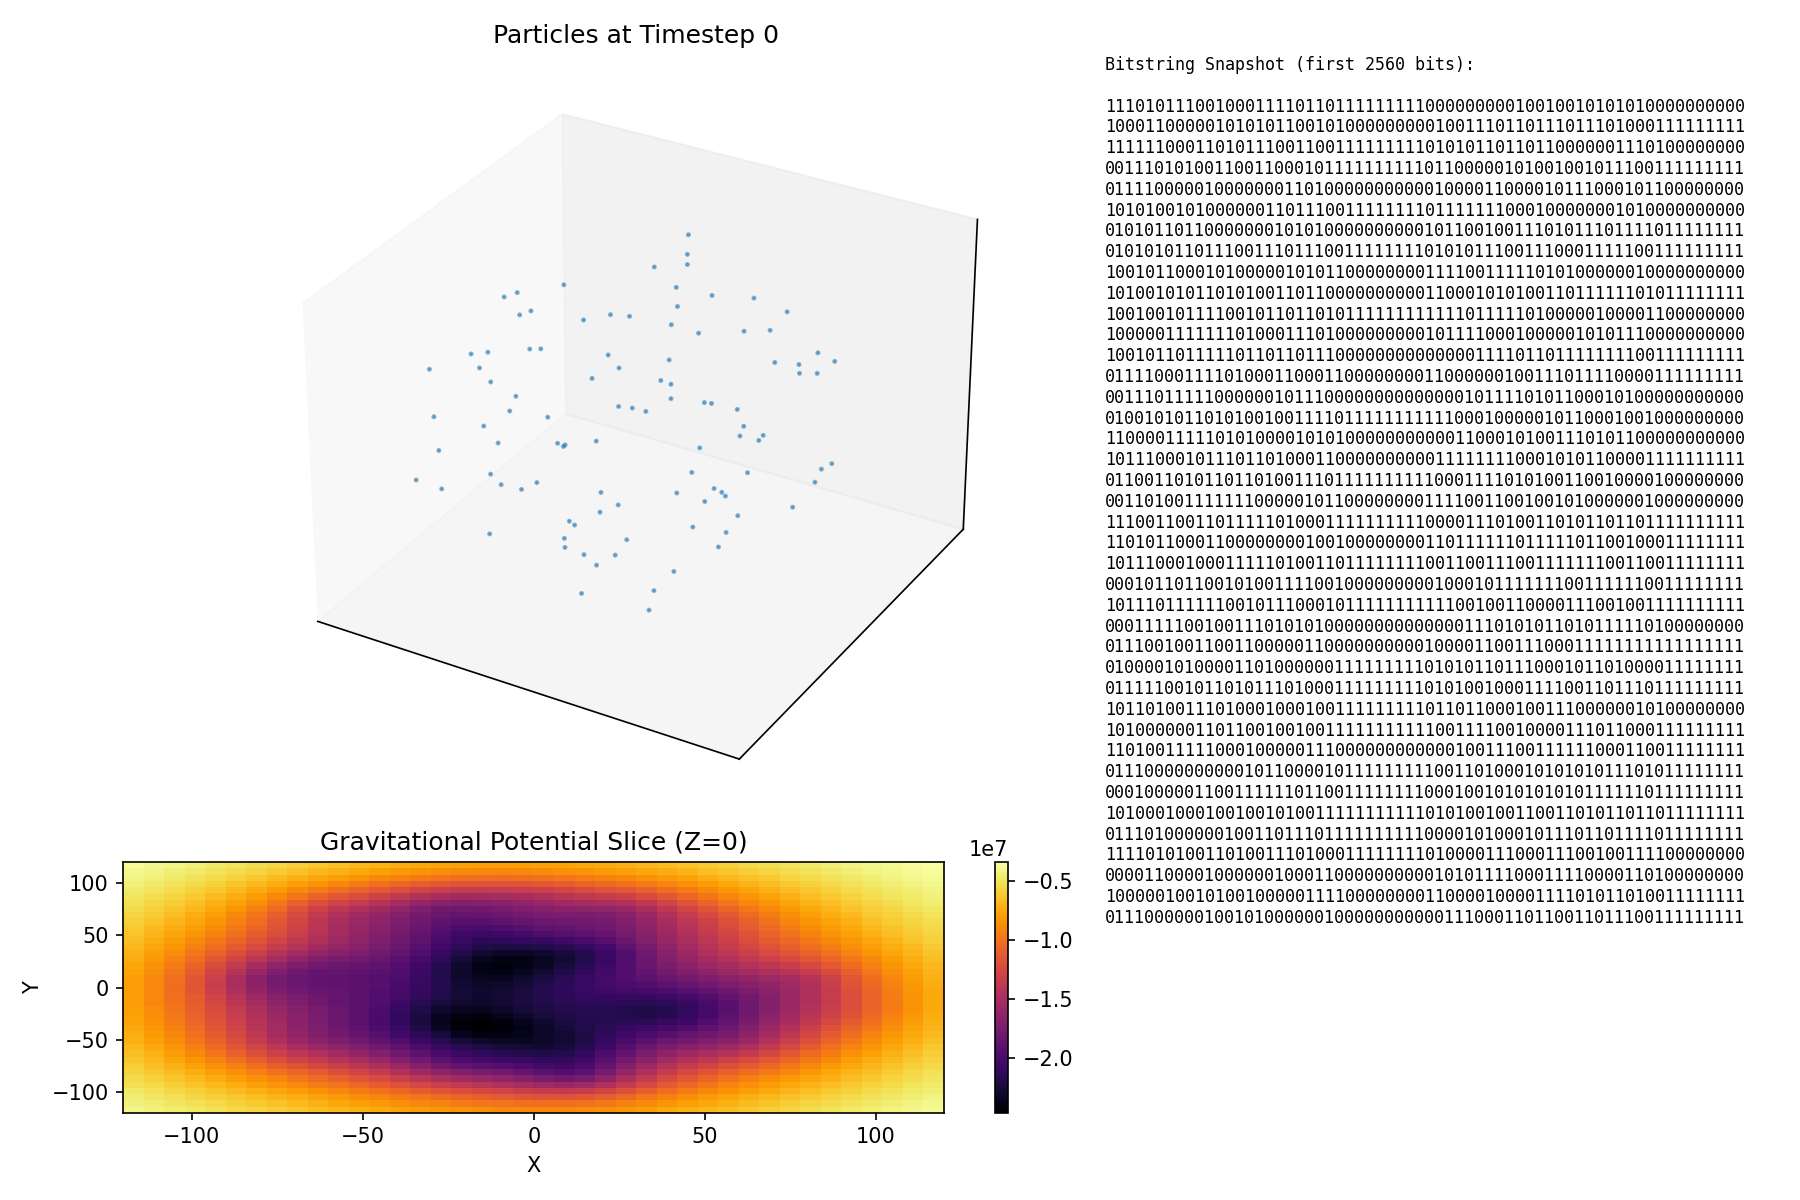
\includegraphics[width=1.0\textwidth]{figures/collapse_0.png}
  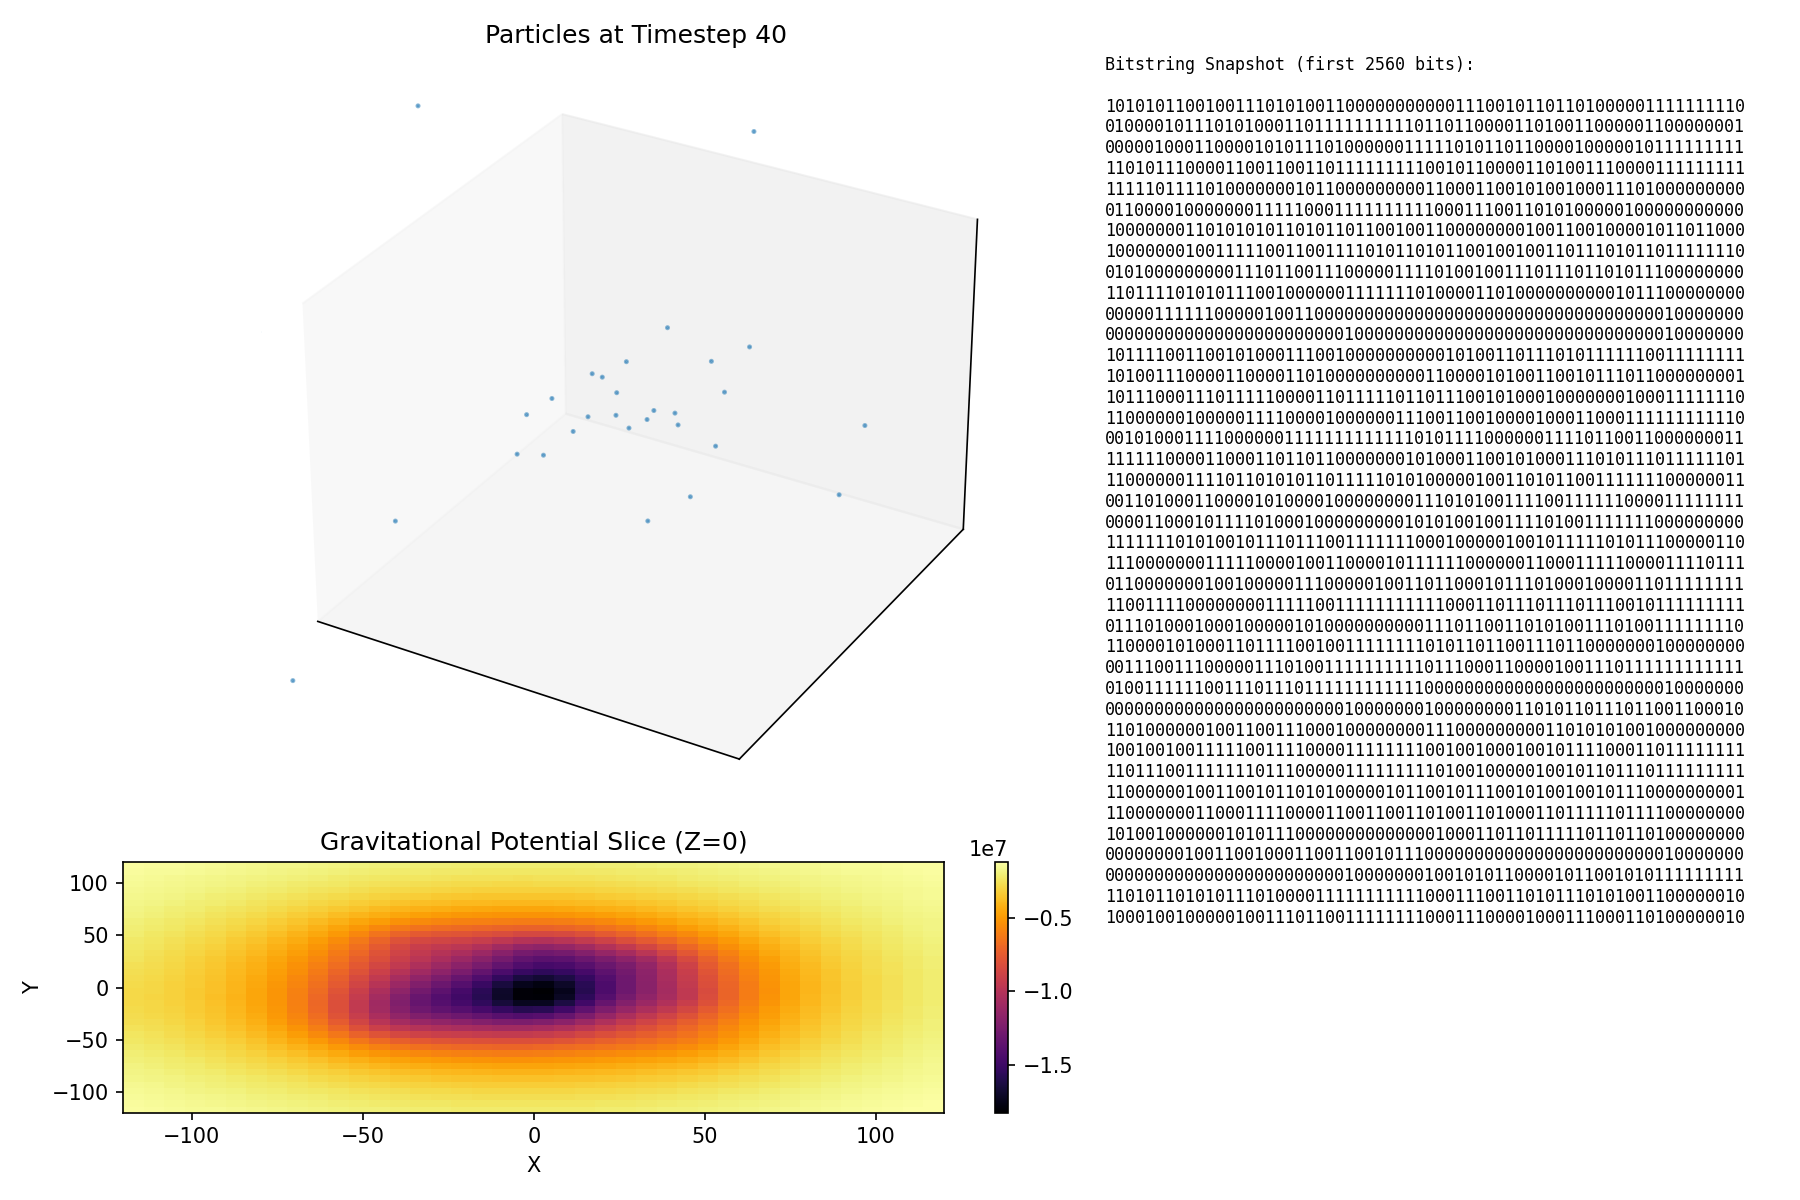
\includegraphics[width=1.0\textwidth]{figures/collapse_40.png}
  \caption{Collapsing spacetime geometry. As entropy decreases, structure shrinks toward a point.}
  \label{fig:vanishing_entropy}
\end{figure}

\section{Conclusion and Future Work}

We have shown that low-entropy informational states necessarily correspond to geometric singularities. This creates an absolute informational scale for entropy, anchored at zero. Future work will model entropy increase as emergent spacetime expansion, simulate structure formation, and explore whether entropy acts as a driver of geometric complexity.

\appendix
\section{Appendix: Bitstring Encoding}

\begin{itemize}
  \item Quantize floating point: $\mathbb{R} \to \mathbb{Z}$
  \item Serialize integers to binary
  \item Concatenate to $b \in \{0,1\}^L$
\end{itemize}

Entropy of $b$:
\[
  H(b) = -p_0 \log_2 p_0 - p_1 \log_2 p_1
\]
where $p_0$, $p_1$ are empirical frequencies.

\section*{References}
\begin{thebibliography}{9}
  \bibitem{Bekenstein1973} J. D. Bekenstein, "Black Holes and Entropy," \textit{Phys. Rev. D} \textbf{7}, 2333 (1973).
  \bibitem{Hawking1975} S. W. Hawking, "Particle Creation by Black Holes," \textit{Commun. Math. Phys.} \textbf{43}, 199 (1975).
\end{thebibliography}

\end{document}
